	\subsection{UC 5 - Gestione dispositivi}
		
		\begin{figure}[H]
			\centering
			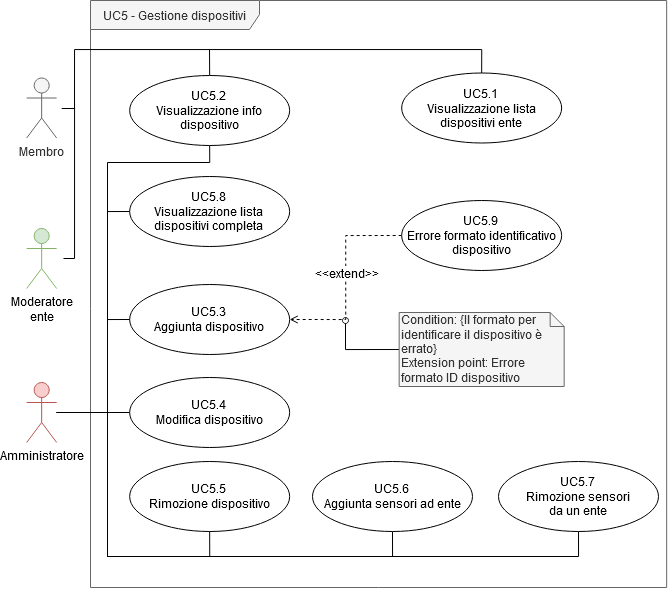
\includegraphics[scale=0.60]{res/images/uc5}
			\caption{Diagramma che riassume la gestione dei dispositivi con cui può interagire l'utente nella web app.}
		\end{figure}
		
		\begin{itemize}
			\item \textbf{attori primari:} membro, moderatore ente, amministratore;
			\item \textbf{descrizione:} l'utente può gestire i dispositivi a cui ha accesso a livello di permessi ed eseguire aggiunte, modifiche o rimozioni;
			\item \textbf{precondizione:} l'utente è autenticato e naviga nella gestione dispositivi del sistema;
			\item \textbf{postcondizione:} l'utente ha visualizzato o gestito i dispositivi;
			\item \textbf{scenario principale:}
			\begin{enumerate}
				\item{l'utente naviga all'interno della gestione dispositivi del sistema;}
				\item{l'utente visualizza o gestisce i dispositivi a cui ha accesso.}
			\end{enumerate}
		\end{itemize}


			\subsubsection{UC 5.1 - Visualizzazione lista dispositivi ente}
			\begin{itemize}
				\item \textbf{attori primari:} membro, moderatore ente;
				\item \textbf{descrizione:} l'utente può visualizzare una lista con ID, nome, numero sensori e nome ente per ogni dispositivo abilitato per il proprio ente;
				\item \textbf{precondizione:} l'utente naviga nella gestione dispositivi del sistema;
				\item \textbf{postcondizione:} l'utente ha visualizzato i dispositivi;
				\item \textbf{scenario principale:}
				\begin{enumerate}
					\item{l'utente visualizza i dispositivi abilitati per il proprio ente.}
				\end{enumerate}
			\end{itemize}

			\subsubsection{UC 5.2 - Visualizza info dispositivo}
			\begin{itemize}
				\item \textbf{attori primari:} membro, moderatore ente, amministratore;
				\item \textbf{descrizione:} l'utente può visualizzare ID, nome, frequenza di aggiornamento dei dati e dati dei sensori in forma tabellare o grafica riguardanti il dispositivo selezionato;
				\item \textbf{precondizione:} l'utente naviga nella gestione dispositivi del sistema;
				\item \textbf{postcondizione:} l'utente ha visualizzato le informazioni del dispositivo selezionato;
				\item \textbf{scenario principale:}
				\begin{enumerate}
					\item{l'utente seleziona il dispositivo dalla lista dispositivi;}
					\item{l'utente visualizza le informazioni del dispositivo.}
				\end{enumerate}
			\end{itemize}

			\subsubsection{UC 5.3 - Aggiunta dispositivo}
			\begin{itemize}
				\item \textbf{attori primari:} amministratore;
				\item \textbf{descrizione:} l'utente può aggiungere, e quindi censire, un nuovo dispositivo nel sistema;
				\item \textbf{precondizione:} l'utente naviga nella gestione dispositivi del sistema;
				\item \textbf{postcondizione:} l'utente ha aggiunto un nuovo dispositivo al sistema;
				\item \textbf{scenario principale:}
				\begin{enumerate}
					\item{l'utente deve inserire dei campi obbligatori per aggiungere un nuovo dispositivo;}
					\item{l'utente compila il campo \textit{identificativo dispositivo} (UC 5.3.1);}
					\item{l'utente compila il campo \textit{nome dispositivo} (UC 5.3.2);}
					\item{l'utente compila il campo \textit{tempo di frequenza ricezione dati} (UC 5.3.3);}
					\item{l'utente compila il campo \textit{dati sensori}( UC 5.3.4);}
					\item{l'utente ha aggiunto un nuovo dispositivo al sistema;}
					\item{l'utente compila il campo \textit{gateway}(UC 5.3.5).}
				\end{enumerate}
				\item \textbf{estensioni:}
				\begin{itemize}
					\item dispositivo non valido (UC 5.9).
				\end{itemize}
			\end{itemize}

				\paragraph{UC 5.3.1 - Inserimento identificativo dispositivo}
				\begin{itemize}
					\item \textbf{attori primari:} amministratore;
					\item \textbf{descrizione:} per proseguire nella aggiunta di un nuovo dispositivo, l'utente deve inserire l'identificativo del dispositivo. Il campo è obbligatorio;
					\item \textbf{precondizione:} l'utente sta inserendo le informazioni per aggiungere un nuovo dispositivo;
					\item \textbf{postcondizione:} l'utente ha compilato un campo richiesto;
					\item \textbf{scenario principale:}
					\begin{enumerate}
						\item{l'utente compila il campo \textit{identificativo dispositivo}.}
					\end{enumerate}
				\end{itemize}

				\paragraph{UC 5.3.2 - Inserimento nome dispositivo}
				\begin{itemize}
					\item \textbf{attori primari:} amministratore;
					\item \textbf{descrizione:} per proseguire nella aggiunta di un nuovo dispositivo, l'utente deve inserire un nome con cui associare il dispositivo. Il campo è obbligatorio;
					\item \textbf{precondizione:} l'utente sta inserendo le informazioni per aggiungere un nuovo dispositivo;
					\item \textbf{postcondizione:} l'utente ha compilato un campo richiesto;
					\item \textbf{scenario principale:}
					\begin{enumerate}
						\item{l'utente compila il campo \textit{nome dispositivo}.}
					\end{enumerate}
				\end{itemize}

				\paragraph{UC 5.3.3 - Inserimento tempo di frequenza ricezione dati}
				\begin{itemize}
					\item \textbf{attori primari:} amministratore;
					\item \textbf{descrizione:} per proseguire nella aggiunta di un nuovo dispositivo, l'utente deve inserire il tempo di frequenza per la ricezione dati nel sistema. Il campo è obbligatorio;
					\item \textbf{precondizione:} l'utente sta inserendo le informazioni per aggiungere un nuovo dispositivo;
					\item \textbf{postcondizione:} l'utente ha compilato un campo richiesto;
					\item \textbf{scenario principale:}
					\begin{enumerate}
						\item{l'utente compila il campo \textit{tempo di frequenza ricezione dati}.}
					\end{enumerate}
				\end{itemize}

				\paragraph{UC 5.3.4 - Inserimento dati sensori}
				\begin{itemize}
					\item \textbf{attori primari:} amministratore;
					\item \textbf{descrizione:} per proseguire nella aggiunta di un nuovo dispositivo, l'utente deve inserire i dati dei sensori del dispositivo di cui vuole ricevere letture. Il campo è obbligatorio;
					\item \textbf{precondizione:} l'utente sta inserendo le informazioni per aggiungere un nuovo dispositivo;
					\item \textbf{postcondizione:} l'utente ha compilato un campo richiesto;
					\item \textbf{scenario principale:}
					\begin{enumerate}
						\item{l'utente compila il campo \textit{dati sensori}.}
					\end{enumerate}
				\end{itemize}

				\paragraph{UC 5.3.5 - Inserimento nome gateway}
				\begin{itemize}
					\item \textbf{attori primari:} amministratore;
					\item \textbf{descrizione:} per proseguire nella aggiunta di un nuovo dispositivo, l'utente deve selezionare il gateway da una lista;
					\item \textbf{precondizione:} l'utente sta inserendo le informazioni per aggiungere un nuovo dispositivo;
					\item \textbf{postcondizione:} l'utente ha compilato un campo richiesto;
					\item \textbf{scenario principale:}
					\begin{enumerate}
						\item{l'utente seleziona il \textit{gateway} da una lista.}
					\end{enumerate}
				\end{itemize}

			\subsubsection{UC 5.4 - Modifica dispositivo}
			\begin{itemize}
				\item \textbf{attori primari:} amministratore;
				\item \textbf{descrizione:} l'utente modifica i dispositivi che gli interessano e la nuova configurazione viene gestita dal sistema;
				\item \textbf{precondizione:} l'utente naviga nella gestione dispositivi del sistema e ha almeno un dispositivo disponibile;
				\item \textbf{postcondizione:} l'utente ha modificato il dispositivo selezionato;
				\item \textbf{scenario principale:}
				\begin{enumerate}
					\item{l'utente seleziona un dispositivo da modificare;}
					\item{l'utente modifica il campo \textit{nome dispositivo} (UC 5.4.1);}
					\item{l'utente modifica il campo \textit{tempo di frequenza ricezione dati} (UC 5.4.2);}
					\item{l'utente modifica i \textit{dati sensori} (UC 5.4.3);}
					\item{l'utente modifica il campo \textit{gateway} (UC 5.4.4);}
					\item{l'utente ha modificato il dispositivo selezionato.}
				\end{enumerate}
			\end{itemize}

			% ndr: da come ha detto Alex, sarebbe da fare una roba che prima modifica tutti i dispositivi e poi c'è un tasto di conferma una volta che tutto è stato modificato. A livello DB si può aggiungere una tabella per gestire i dispositivi modificati e poi controllare quando è stata sovrascritta l'ultima configurazione a un gateway.

				\paragraph{UC 5.4.1 - Modifica nome dispositivo}
				\begin{itemize}
					\item \textbf{attori primari:} amministratore;
					\item \textbf{descrizione:} per proseguire nella modifica di un dispositivo, l'utente deve modificare il nome con cui associare il dispositivo. Il campo è obbligatorio;
					\item \textbf{precondizione:} l'utente sta modificando le informazioni di dispositivo già censito;
					\item \textbf{postcondizione:} l'utente ha compilato un campo richiesto;
					\item \textbf{scenario principale:}
					\begin{enumerate}
						\item{l'utente compila il campo \textit{nome dispositivo}.}
					\end{enumerate}
				\end{itemize}

				\paragraph{UC 5.4.2 - Modifica tempo di frequenza ricezione dati}
				\begin{itemize}
					\item \textbf{attori primari:} amministratore;
					\item \textbf{descrizione:} per proseguire nella modifica di un dispositivo, l'utente deve modificare il tempo di frequenza per la ricezione dati nel sistema. Il campo è obbligatorio;
					\item \textbf{precondizione:} l'utente sta modificando le informazioni di dispositivo già censito;
					\item \textbf{postcondizione:} l'utente ha compilato un campo richiesto;
					\item \textbf{scenario principale:}
					\begin{enumerate}
						\item{l'utente compila il campo \textit{tempo di frequenza ricezione dati}.}
					\end{enumerate}
				\end{itemize}

				\paragraph{UC 5.4.3 - Modifica dati sensori}
				\begin{itemize}
					\item \textbf{attori primari:} amministratore;
					\item \textbf{descrizione:} per proseguire nella modifica di un dispositivo, l'utente deve modificare i dati dei sensori del dispositivo di cui vuole ricevere letture. Il campo è obbligatorio;
					\item \textbf{precondizione:} l'utente sta modificando le informazioni di dispositivo già censito;
					\item \textbf{postcondizione:} l'utente ha compilato un campo richiesto;
					\item \textbf{scenario principale:}
					\begin{enumerate}
						\item{l'utente compila il campo \textit{dati sensori}.}
					\end{enumerate}
				\end{itemize}

				\paragraph{UC 5.4.4 - Modifica nome gateway}
				\begin{itemize}
					\item \textbf{attori primari:} amministratore;
					\item \textbf{descrizione:} per proseguire nella modifica di un dispositivo, l'utente deve modificare il nome del \glock{gateway} selezionandolo da una lista;
					\item \textbf{precondizione:} l'utente sta modificando le informazioni di dispositivo già censito;
					\item \textbf{postcondizione:} l'utente ha compilato un campo richiesto;
					\item \textbf{scenario principale:}
					\begin{enumerate}
						\item{l'utente seleziona il \textit{gateway} da una lista.}
					\end{enumerate}
				\end{itemize}

			\subsubsection{UC 5.5 - Rimozione dispositivo}
			\begin{itemize}
				\item \textbf{attori primari:} amministratore;
				\item \textbf{descrizione:} l'utente può rimuovere dal sistema un dispositivo in base ai dispositivi censiti a sistema;
				\item \textbf{precondizione:} l'utente naviga nella gestione dispositivi del sistema e ha almeno un dispositivo disponibile;
				\item \textbf{postcondizione:} l'utente ha rimosso il dispositivo selezionato dal sistema;
				\item \textbf{scenario principale:}
				\begin{enumerate}
					\item{l'utente seleziona un dispositivo da rimuovere tra quelli disponibili;}
					\item{l'utente ha rimosso il dispositivo selezionato dal sistema.}
				\end{enumerate}
			\end{itemize}

			\subsubsection{UC 5.6 - Aggiunta sensori ad ente}
			\begin{itemize}
				\item \textbf{attori primari:} amministratore;
				\item \textbf{descrizione:} l'utente può aggiungere i permessi di lettura e monitoraggio dei dati di un dispositivo a un particolare ente;
				\item \textbf{precondizione:} l'utente naviga nella gestione dispositivi del sistema;
				\item \textbf{postcondizione:} l'utente ha concesso il monitoraggio di un sensore ad un ente;
				\item \textbf{scenario principale:}
				\begin{enumerate}
					\item{l'utente seleziona un sensore di un particolare dispositivo e lo abilita a un ente;}
					\item{l'utente ha permesso il monitoraggio del sensore all'ente selezionato.}
				\end{enumerate}
			\end{itemize}

			\subsubsection{UC 5.7 - Rimozione sensori da un ente}
			\begin{itemize}
				\item \textbf{attori primari:} amministratore;
				\item \textbf{descrizione:} l'utente può rimuovere i permessi di monitoraggio dei dati del dispositivo selezionato all'ente selezionato;
				\item \textbf{precondizione:} l'utente visualizza le informazioni del dispositivo;
				\item \textbf{postcondizione:} l'utente ha rimosso il permesso di monitoraggio del dato del dispositivo all'ente selezionato;
				\item \textbf{scenario principale:}
				\begin{enumerate}
					\item{l'utente rimuove un sensore di un particolare dispositivo a un ente;}
					\item{l'utente ha rimosso il permesso di monitoraggio del sensore all'ente selezionato.}
				\end{enumerate}
			\end{itemize}

			\subsubsection{UC 5.8 - Visualizzazione lista dispositivi completa}
			\begin{itemize}
				\item \textbf{attori primari:} amministratore;
				\item \textbf{descrizione:} l'utente può visualizzare una lista con ID, nome, numero di sensori e nome dell'ente per ogni dispositivo presente nel sistema;
				\item \textbf{precondizione:} l'utente naviga nella gestione dispositivi del sistema;
				\item \textbf{postcondizione:} l'utente ha visualizzato la lista di tutti i dispositivi;
				\item \textbf{scenario principale:}
				\begin{enumerate}
					\item{l'utente visualizza tutti i dispositivi presenti nel sistema.}
				\end{enumerate}
			\end{itemize}

			s
